\section{Kommutierendes Diagramm}

	\begin{figure}[!h]
		\centering
		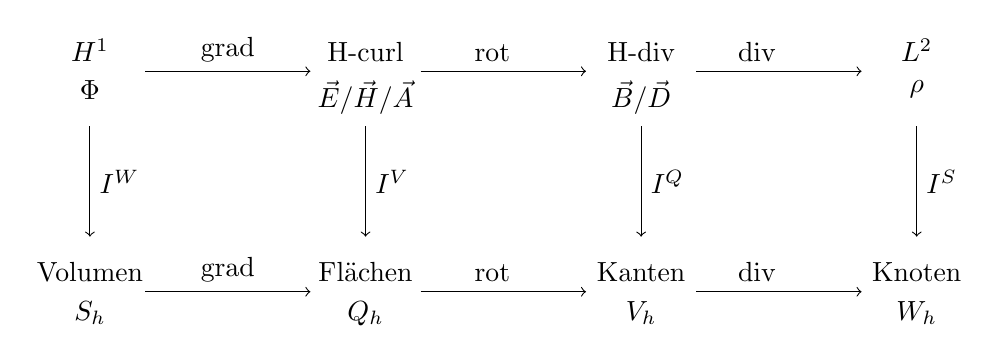
\begin{tikzpicture}[scale=2.8]

		\draw[->] (0.25,1) -- (1,1);
		\draw[->] (1.5,1) -- (2.25,1);
		\draw[->] (2.75,1) -- (3.5,1);

		\node at (0.625,1) [above] {grad};
		\node at (1.825,1) [above] {rot};
		\node at (3.025,1) [above] {div};

		\node at (0,1) [above] {$H^1$};
		\node at (0,1) [below] {$\Phi$};
		\node at (1.25,1) [below] {$\vec{E}$/$\vec{H}$/$\vec{A}$};
		\node at (1.25,1) [above] {H-curl};
		\node at (2.5,1) [above] {H-div};
		\node at (2.5,1) [below] {$\vec{B}$/$\vec{D}$};
		\node at (3.75,1) [above] {$L^2$};
		\node at (3.75,1) [below] {$\rho$};


		\draw[->] (0,0.75) -- (0,0.25);
		\draw[->] (1.25,0.75) -- (1.25,0.25);
		\draw[->] (2.5,0.75) -- (2.5,0.25);
		\draw[->] (3.75,0.75) -- (3.75,0.25);

		\node at (0,0.5) [right] {$I^W$};
		\node at (1.25,0.5) [right] {$I^V$};
		\node at (2.5,0.5) [right] {$I^Q$};
		\node at (3.75,0.5) [right] {$I^S$};

		\draw[->] (0.25,0) -- (1,0);
		\draw[->] (1.5,0) -- (2.25,0);
		\draw[->] (2.75,0) -- (3.5,0);

		\node at (0.625,0) [above] {grad};
		\node at (1.825,0) [above] {rot};
		\node at (3.025,0) [above] {div};

		\node at (0,0) [above] {Volumen};
		\node at (0,0) [below] {$S_h$};
		\node at (1.25,0) [above] {Fl\"achen};
		\node at (1.25,0) [below] {$Q_h$};
		\node at (2.5,0) [above] {Kanten};
		\node at (2.5,0) [below] {$V_h$};
		\node at (3.75,0) [above] {Knoten};
		\node at (3.75,0) [below] {$W_h$};

		\end{tikzpicture}
	\end{figure}
	Mit $I^W$: Knoteninterpolation, $I^V$: Kanteninterpolation, $I^Q$: Fl\"acheninterpolation und $I^S$: $L_2$ Projektion.